\documentclass[12pt,a4paper,hidelinks]{article}

\usepackage{ulem}
\usepackage{incgraph}
\usepackage{tikz}
\usepackage{hyperref}

\newcommand{\leftcoordinate}{-15cm}
\usetikzlibrary{mindmap,shadows,calendar,fadings,arrows.meta}
\tikzset{todo/.append style={annotation,above,concept color=white,draw=black,text width=2cm,align=center}}
\hypersetup{
    colorlinks=false,
    linkcolor=black,
    filecolor=magenta,      
    urlcolor=cyan,
}

\begin{document}
\begin{inctext}
    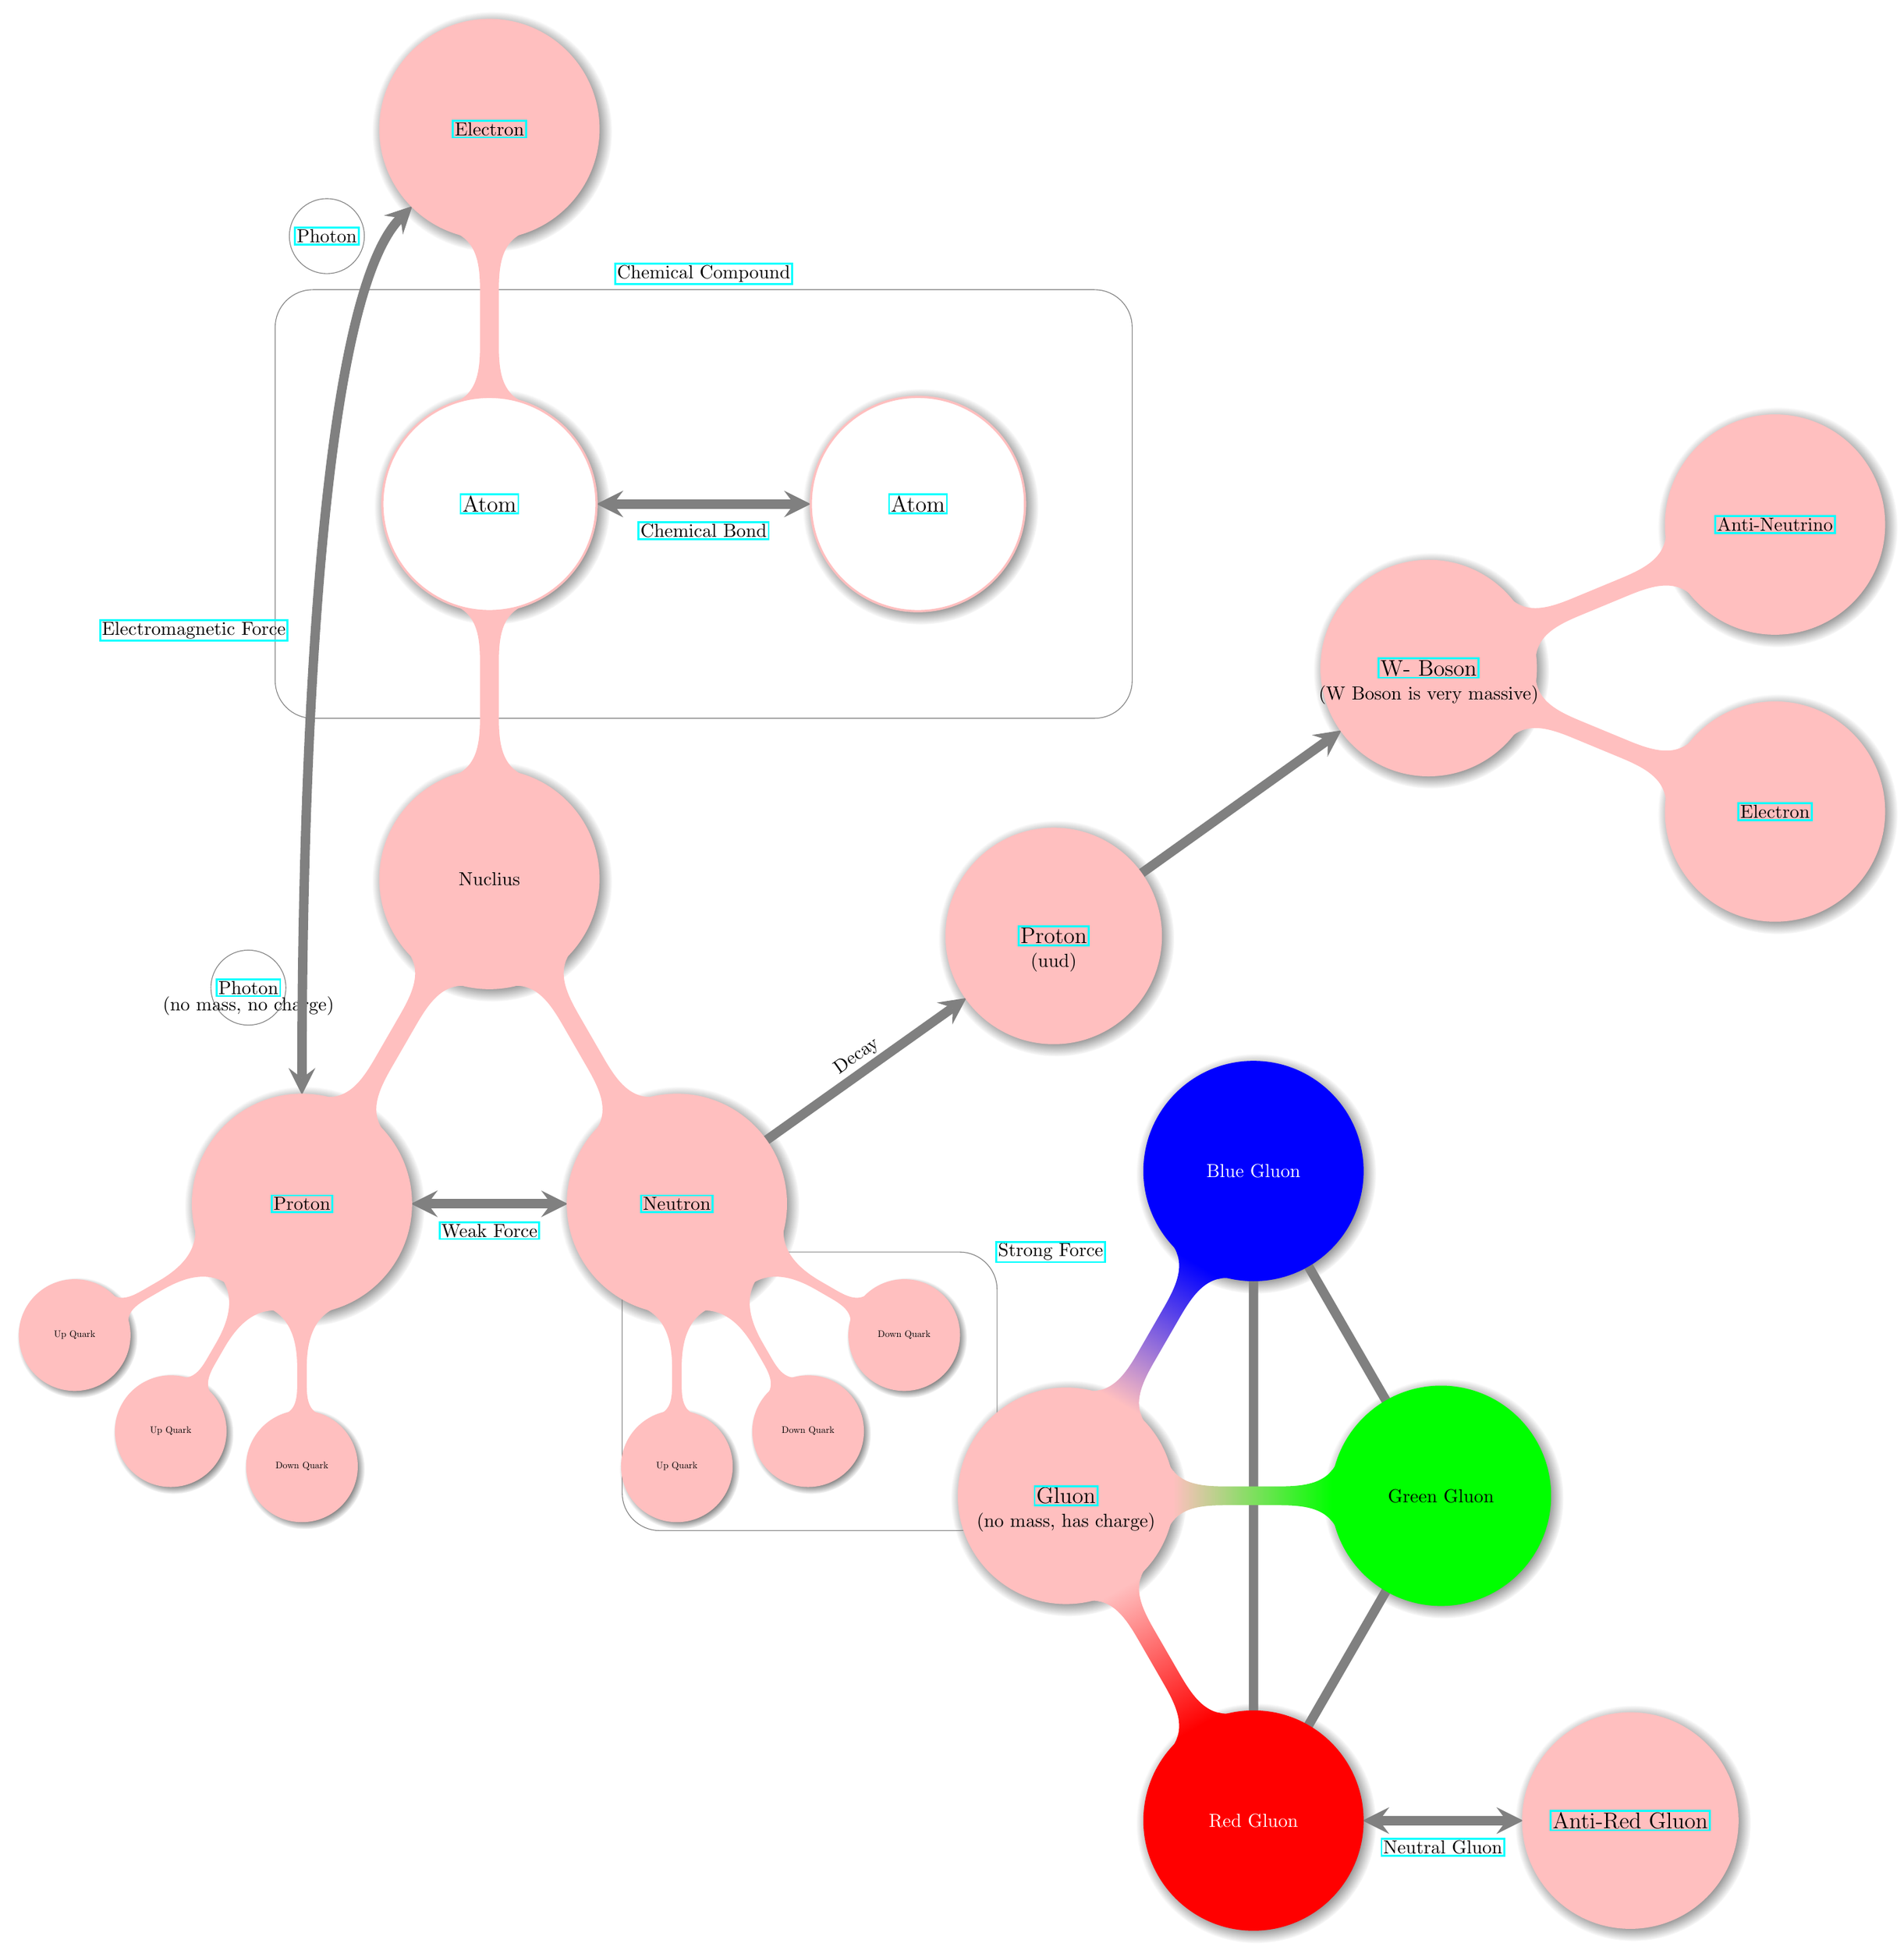
\begin{tikzpicture}
        \pgfdeclarelayer{background}
        \pgfdeclarelayer{foreground}
        \pgfsetlayers{background,main,foreground}
        % ------------------------ declare mindmap ------------------------ %
        \begin{scope}[
                mindmap,
                grow cyclic,
                concept color=pink,
                every node/.append style={concept,circular drop shadow,text width=4cm},
                level 1/.append style={sibling angle=360/2},
                every child/.append style={level distance=7cm,font=\fontsize{10pt}{12pt}}
            ]
            \node[root concept, fill=white](atom){
                \href{https://en.wikipedia.org/wiki/Atom}{Atom}
            }
            child{
                    node{
                            Nuclius
                        }
                    child{
                            node(proton){
                                    \href{https://en.wikipedia.org/wiki/Proton}{Proton}
                                }
                            child[scale=.7]{
                                    node[scale=.5]{
                                            Up Quark
                                        }
                                }
                            child[scale=.7]{
                                    node[scale=.5]{
                                            Up Quark
                                        }
                                }
                            child[scale=.7]{
                                    node[scale=.5]{
                                            Down Quark
                                        }
                                }
                        }
                    child{
                            node(neutron){
                                    \href{https://en.wikipedia.org/wiki/Neutron}{Neutron}
                                }
                            child[scale=.7]{
                                    node[scale=.5](upq){
                                            Up Quark
                                        }
                                }
                            child[scale=.7]{
                                    node[scale=.5]{
                                            Down Quark
                                        }
                                }
                            child[scale=.7]{
                                    node[scale=.5](doq){
                                            Down Quark
                                        }
                                }
                        }
                }
            child{
                    node(electron){
                            \href{https://en.wikipedia.org/wiki/Electron}{Electron}
                        }
                }
            ;
            \node[root concept, fill=white,xshift=8cm](atom2) at (atom){
                \href{https://en.wikipedia.org/wiki/Atom}{Atom}
            };
            \node[root concept,xshift=2cm,yshift=-3cm](gluon) at (doq.east){
                \href{https://en.wikipedia.org/wiki/Gluon}{Gluon}
            }
            child[sibling angle=60,concept color=red,white]{
                    node(redg){
                            Red Gluon
                        }
                }
            child[sibling angle=60,concept color=green]{
                    node(greeng){
                            Green Gluon
                        }
                }
            child[sibling angle=60,concept color=blue,white]{
                    node(blueg){
                            Blue Gluon
                        }
                }
            ;
            \node[root concept,xshift=5cm](antig) at (redg.east){
                \href{https://en.wikipedia.org/wiki/Color_charge}{Anti-Red Gluon}
            };
            \node[root concept,xshift=5cm,yshift=5cm](proton2) at (neutron.east){
                \href{https://en.wikipedia.org/wiki/Proton}{Proton}
            };
            \node[root concept,xshift=5cm,yshift=5cm](wboson) at (proton2.east){
                \href{https://en.wikipedia.org/wiki/W_and_Z_bosons}{W- Boson}
            }
            child[sibling angle=45]{
                    node{
                            \href{https://en.wikipedia.org/wiki/Electron}{Electron}
                        }
                }
            child[sibling angle=45]{
                    node{
                            \href{https://en.wikipedia.org/wiki/Neutrino}{Anti-Neutrino}
                        }
                }
            ;
        \end{scope}
        % ------------------------ background ------------------------ %
        \begin{pgfonlayer}{background}
            \draw[rounded corners=20pt,gray] (atom)+(-4,4) node[xshift=8cm,yshift=.3cm,black]{\href{https://en.wikipedia.org/wiki/Chemical_compound}{Chemical Compound}} rectangle (12,-4)+(atom2);
            \draw[gray,rounded corners=20pt] (upq.west)+(0,-1.2) rectangle +(7,4)node[black,xshift=1cm]{\href{https://en.wikipedia.org/wiki/Strong_interaction}{Strong Force}};
            \draw[gray] (proton.north)+(-1,2) node[black](photon){\href{https://en.wikipedia.org/wiki/Photon}{Photon}} circle (.7cm);
            \node[yshift=-.1cm] at(photon.south){(no mass, no charge)};
            \draw[gray] (electron.west)+(-1,-2) node[black]{\href{https://en.wikipedia.org/wiki/Photon}{Photon}} circle (.7cm);
            \draw[{stealth[width=15pt,length=10pt]}-{stealth[width=15pt,length=10pt]},line width=5pt,color=gray](proton)--node[yshift=-.5cm,black]{\href{https://en.wikipedia.org/wiki/Nuclear_force}{Weak Force}}(neutron);
            \draw[{stealth[width=15pt,length=10pt]}-{stealth[width=15pt,length=10pt]},line width=5pt,color=gray](proton.north) .. controls +(0,3) and +(-2,-2) .. node[xshift=-2.3cm,black]{\href{https://en.wikipedia.org/wiki/Electromagnetism}{Electromagnetic Force}}(electron.south west);
            \draw[{stealth[width=15pt,length=10pt]}-{stealth[width=15pt,length=10pt]},line width=5pt,color=gray](atom)--node[yshift=-.5cm,black]{\href{https://en.wikipedia.org/wiki/Chemical_bond}{\href{https://en.wikipedia.org/wiki/Chemical_bond}{Chemical Bond}}}(atom2);
            \draw[{stealth[width=15pt,length=10pt]}-{stealth[width=15pt,length=10pt]},line width=5pt,color=gray](redg)--node[yshift=-.5cm,black]{\href{https://en.wikipedia.org/wiki/Chemical_bond}{\href{https://en.wikipedia.org/wiki/Chemical_bond}{Neutral Gluon}}}(antig);
            \draw[-,line width=5pt,color=gray](redg)--(blueg)--(greeng)--(redg);
            \draw[-{stealth[width=15pt,length=10pt]},line width=5pt,color=gray](neutron)--node[black,yshift=.3cm,sloped]{Decay}(proton2);
            \draw[-{stealth[width=15pt,length=10pt]},line width=5pt,color=gray](proton2)--(wboson);
        \end{pgfonlayer}
        % ------------------------ foreground ------------------------ %
        \begin{pgfonlayer}{foreground}
            % \node[text width=1cm, text height=1cm,yshift=-1cm] at (main) {
            %     \includegraphics[width=1cm,height=1cm]{../image/book.png}
            % };
            \node[yshift=-.5cm] at(gluon) {(no mass, has charge)};
            \node[yshift=-.5cm] at(proton2) {(uud)};
            \node[yshift=-.5cm] at(wboson) {(W Boson is very massive)};
        \end{pgfonlayer}
    \end{tikzpicture}
\end{inctext}
%------------------------------------------------------------ List ------------------------------------------------------------%
\noindent
\href{https://www.youtube.com/watch?v=ehHoOYqAT_U}{What’s the smallest thing in the universe?}\\
\href{https://www.youtube.com/watch?v=xZqID1zSm0k}{Why \& How do the 4 fundamental forces of nature work?}
\end{document}